\section{Sample execution}
\label{sec:sample-execution}
% DEBORA
In this section we will see some sample execution from natural language to the final answer. Let's start with a simple example:

\begin{enumerate}
\item "\textit{Who is the chief financial officer of Apple?}"
As we can see from the \textit{Fig.2} in the Section \ref{sec:architecture}, our input is an english natural language question.  The parsing algorithm described in section \ref{sec:parsing}, gives us a LTAG. Next, syntactic and semantic composition rules apply in tandem in order to construct a LTAG and a DUDES:
\begin{itemize}
\item \textbf{LTAG}
\medskip
\begin{center}
\begin{tabular}{ p{10em} p{10em} p{10em} }
	\label{tbl:grammar.example1}
	\begin{center}{(1)} \end{center}
	\begin{center}
		\begin{tikzpicture}
		\Tree [.S [.DP$_1\downarrow$ ] [.VP [.V is ] DP$_2\downarrow$ ] ]	
		\end{tikzpicture}
	\end{center}

	&
	
	\begin{center}{(2)} \end{center}
	\begin{center}
		\begin{tikzpicture}
		\Tree [.S [.DP  [.PRN who ] ] [.VP [.V is ] DP$_2\downarrow$ ] ]	
		\end{tikzpicture}
	\end{center}
	
	&
	
	\begin{center}{(3)} \end{center}
	\begin{center}
		\begin{tikzpicture}
		\Tree [.S [.DP  [.PRN who ] ] [.VP [.V is ] [.DP  [.DET the ] [.NP$_1\downarrow$ ]] ] ]	
		\end{tikzpicture}
	\end{center}
	\\
\end{tabular}
\end{center}
\medskip

\medskip
\begin{center}
\begin{tabular}{ p{10em} p{10em} p{10em} p{10em} }
	\label{tbl:grammar.example1}
		
	\begin{center}{(4)} \end{center}
	\begin{center}
		\begin{tikzpicture}
		\Tree [.S [.DP  [.PRN who ] ] [.VP [.V is ] [.DP  [.DET the ] [.NP [.N \text{chief financial officer} ] [.PP [.P of ] DP$_1\downarrow$ ]]
] ] ]	
		\end{tikzpicture}
	\end{center}
	
	&
	\mbox{}
	&
	\begin{center}{(5)} \end{center}
	\begin{center}
	\begin{tikzpicture}
	\Tree [.S [.DP  [.PRN who ] ] [.VP [.V is ] [.DP  [.DET the ] [.NP [.N \text{chief financial officer} ] [.PP [.P of ] [.DP Apple ] ]]
] ] ]	
		\end{tikzpicture}
	\end{center}
	&
\mbox{}
	\\
\end{tabular}
\end{center}



\medskip

\item \textbf{DUDES} 
\medskip
\begin{center}
\begin{tabular}{ p{10em} }
	\label{tbl:grammar.example1}
	
	\begin{center}
		\begin{tabular}{|c|l|}
			\hline
			\mbox{} & ?x \\ 
			\hline
			\multicolumn{2}{|l|}{
				$hasCFO(y,x)$
			}\\
			\multicolumn{2}{|l|}{
			$y=Apple$
			}\\
			\hline
			\multicolumn{2}{|l|}{
				\mbox{}
			} \\
			\hline
		\end{tabular}
	\end{center}	
	\\
\end{tabular}
\end{center}
\medskip

\end{itemize}
The final step consists in translating this DUDES into a SPARQL query. Here the query generated by this question:
\\
\\
\textit{PREFIX org: $<http://www.semanticweb.org/organization \# >$}
\\
\\
\textit{SELECT DISTINCT ?x \\
\mbox{}\qquad WHERE $\{$ org:Apple org:hasCFO ?x $\}$}
\\

\item "\textit{What is the most valuable company?}"
A special case is the quantifier \textit{the most}. The process for getting the answer is the same of the previous example and the construction of the LTAG is very similar. The particularity of this question is in the semantic representation.
 
\begin{itemize}
\item \textbf{LTAG}
\medskip
\begin{center}
\begin{tabular}{ p{10em} p{10em} p{10em} }
	\label{tbl:grammar.example2}
		
	\mbox{}
	&
	
	\begin{center}
		\begin{tikzpicture}
		\Tree [.S [.DP  [.PRN what ] ] [.VP [.V is ] [.DP  [.DET the ] [.ADJ \text{most valuable} ] [.NP company ]] ] ]	
		\end{tikzpicture}
	\end{center}
		
	&
	
	\mbox{}
	
	\\
\end{tabular}
\end{center}
\medskip

\item \textbf{DUDES}	
\medskip
\begin{center}
\begin{tabular}{ p{10em} }
	\label{tbl:grammar.example1}
	
	\begin{center}
		\begin{tabular}{|c|l|}
			\hline
			\mbox{} & ?x \\ 
			\hline
			\multicolumn{2}{|l|}{
				$marketValue(x,y)$
			}\\
			\multicolumn{2}{|l|}{
				$Company(y)$
			}\\
			\multicolumn{2}{|l|}{
				$MAX(x,y)$
			}\\
			\hline
			\multicolumn{2}{|l|}{
				\mbox{}
			} \\
			\hline
		\end{tabular}
	\end{center}	
	\\
\end{tabular}
\end{center}
\medskip
\end{itemize}
The final translation from DUDES generates the following query:
\\
\\
\textit{PREFIX org: $<http://www.semanticweb.org/organization \# >$}
\\
\\
\textit{SELECT DISTINCT ?x \\
\mbox{}\qquad WHERE $\{$ org:x org:marketValue ?y $\}$\\
\mbox{}\qquad ORDER BY DESC(?y)\\
\mbox{}\qquad OFFSET 0\\
\mbox{}\qquad LIMIT 1}\\
\\



		



\item "\textit{Did Microsoft acquire a company headquartered in Italy?}"
The reader can see the use of the adjunction operation in this example. Below the LTAG, the DUDES and the final SPARQL query:
\begin{itemize}
\item \textbf{LTAG}
\medskip
\begin{center}
\begin{tabular}{ p{10em} p{3em} p{10em} p{3em} p{10em} }
	\label{tbl:grammar.example1}
	\begin{center}{(1)} \end{center}
	\begin{center}
		\begin{tikzpicture}
		\Tree [.S [.DP$_1\downarrow$ ] [.VP [.V acquire ] DP$_2\downarrow$ ] ]	
		\end{tikzpicture}
	\end{center}
	
	&
	\mbox{}
	&

	\begin{center}{(2)} \end{center}
	\begin{center}
		\begin{tikzpicture}
		\Tree [.S [.DP  Microsoft ] [.VP [.V acquire ] DP$_2\downarrow$ ] ]	
		\end{tikzpicture}
	\end{center}
	
	&
	\mbox{}
	&
	
	\begin{center}{(3)} \end{center}
	\begin{center}
		\begin{tikzpicture}
		\Tree [.S [.DP  Microsoft ] [.VP [.V acquire ] [.DP  [.DET a ] [.NP$_1\downarrow$ ]] ] ]	
		\end{tikzpicture}
	\end{center}
	\\
\end{tabular}
\end{center}
\medskip

\medskip
\begin{center}
\begin{tabular}{ p{10em} p{3em} p{10em} p{10em}}
	\label{tbl:grammar.example3}
	\begin{center}{(4)} \end{center}
	\begin{center}
		\begin{tikzpicture}
		\Tree [.S [.DP  Microsoft ] [.VP [.V acquire ] [.DP  [.DET a ] [.NP company ]] ] ]	
		\end{tikzpicture}
	\end{center}
	
	&
	\mbox{}
	&

	\begin{center}{(5)} \end{center}
	\begin{center}
		\begin{tikzpicture}
		\Tree [.S [.DP  Microsoft ] [.VP [.V acquire ] [.DP  [.DET a ] [.NP [ company ] [.ADJPP [.ADJ headquartered ] [.PP [.P in ] DP$_1\downarrow$ ] ]]] ] ]	
		\end{tikzpicture}
	\end{center}
	&
	\mbox{}
	\\
\end{tabular}
\end{center}
\medskip

\medskip
\begin{center}
\begin{tabular}{ p{10em} p{6em} p{10em} p{17em}}
	\label{tbl:grammar.example3}
	
	\begin{center}{(6)} \end{center}
	\begin{center}
		\begin{tikzpicture}
		\Tree [.S [.DP  Microsoft ] [.VP [.V acquire ] [.DP  [.DET a ] [.NP [ company ] [.ADJPP [.ADJ headquartered ] [.PP [.P in ] [.DP Italy ] ] ]]] ] ]	
		\end{tikzpicture}
	\end{center}
	
	&
	\mbox{}
	&
	
	\begin{center}{(7)} \end{center}
	\begin{center}
		\begin{tikzpicture}
		\Tree [.S [.V did ] [.DP  Microsoft ] [.VP [.V acquire ] [.DP  [.DET a ] [.NP [ company ] [.ADJPP [.ADJ headquartered ] [.PP [.P in ] [.DP Italy ] ] ]]] ] ]	
		\end{tikzpicture}
	\end{center}
	&
	\mbox{}
	\\
\end{tabular}
\end{center}
\medskip

\item \textbf{DUDES}
\medskip
\begin{center}
\begin{tabular}{ p{10em} }
	\label{tbl:grammar.example3}
	
	\begin{center}
		\begin{tabular}{|c|l|}
			\hline
			\mbox{} & x \\ 
			\hline
			\multicolumn{2}{|l|}{
			$isAcquiredBy(x,y)$
			}\\
			\multicolumn{2}{|l|}{
			$Company(x)$
			}\\
			\multicolumn{2}{|l|}{
			$y=Microsoft$
			}\\
			\multicolumn{2}{|l|}{
			$hasHeadquarter(x,z)$
			}\\
			\multicolumn{2}{|l|}{
			$z=Italy$
			}\\
			\hline
			\multicolumn{2}{|l|}{
				\mbox{}
			} \\
			\hline
		\end{tabular}
	\end{center}	
	\\
\end{tabular}
\end{center}
\medskip
\end{itemize}
The generated query SPARQL is:
\\
\\
\textit{PREFIX org: $<http://www.semanticweb.org/organization \# >$}
\\
\\
\textit{ASK \\
\mbox{}\qquad WHERE $\{$ ?x org:isAcquiredBy org:Microsoft .\\
\mbox{}\qquad \qquad \qquad ?x org:hasHeadquarter org:Italy
\mbox{}\qquad $\}$ \\
\mbox{}\qquad ORDER BY DESC(?y)\\
\mbox{}\qquad OFFSET 0\\
\mbox{}\qquad LIMIT 1}\\
\\ 

\end{enumerate}